\documentclass[border=5mm,tikz]{standalone}
\usepackage{mwe}
\usepackage{tikz}
\begin{document}

% https://tex.stackexchange.com/questions/233010/drawing-a-labeled-cube-using-tikz
% https://tex.stackexchange.com/questions/282044/how-to-fill-a-circle-node
%
% note on colors: gray!20 is a lighter gray

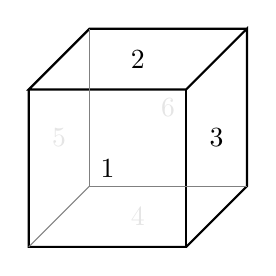
\begin{tikzpicture}
  \draw[thick](2,2,0)--(0,2,0)--(0,2,2)--(2,2,2)--(2,2,0)--(2,0,0)--(2,0,2)--(0,0,2)--(0,2,2);
  \draw[thick](2,2,2)--(2,0,2);
  \draw[gray](2,0,0)--(0,0,0)--(0,2,0);
  \draw[gray](0,0,0)--(0,0,2);
  \draw(1,1,2) node{1};
  \draw(1,2,1) node{2};
  \draw(2,1,1) node{3};
  \draw[gray!20](1,0,1) node{4};
  \draw[gray!20](0,1,1) node{5};
  \draw[gray!20](1,1,0) node{6};
\end{tikzpicture}

\pagebreak

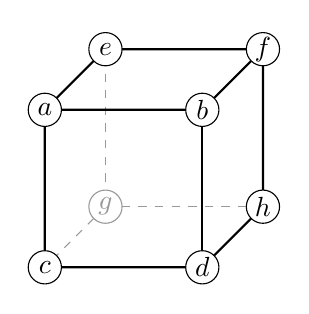
\begin{tikzpicture}
\def\colr{gray!80};

\draw[\colr,dashed](2,0,0)--(0,0,0)--(0,2,0);
\draw[\colr,dashed](0,0,0)--(0,0,2);
\draw[thick](2,2,0)--(0,2,0)--(0,2,2)--(2,2,2)--(2,2,0)--(2,0,0)--(2,0,2)--(0,0,2)--(0,2,2);
\draw[thick](2,2,2)--(2,0,2);

\node[circle,draw=black,fill=white,minimum size=12pt, label=center:{$a$}] at (0,2,2) {};
\node[circle,draw=black,fill=white,minimum size=12pt, label=center:{$b$}] at (2,2,2) {};
\node[circle,draw=black,fill=white,minimum size=12pt, label=center:{$c$}] at (0,0,2) {};
\node[circle,draw=black,fill=white,minimum size=12pt, label=center:{$d$}] at (2,0,2) {};

\node[circle,draw=black,fill=white,minimum size=12pt, label=center:{$e$}] at (0,2,0) {};
\node[circle,draw=black,fill=white,minimum size=12pt,
label=center:{$f$}] at (2,2,0) {};
\node[circle,draw=\colr,fill=white,minimum size=12pt, label=center:{\color{\colr}$g$}] at (0,0,0) {};
\node[circle,draw=black,fill=white,minimum size=12pt, label=center:{$h$}] at (2,0,0) {};

\end{tikzpicture}

\pagebreak

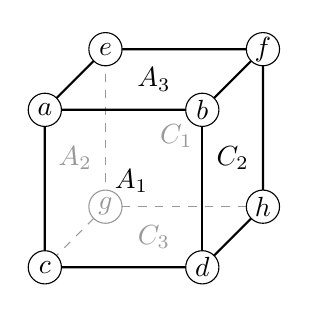
\begin{tikzpicture}
\def\colr{gray!80};

\draw[\colr,dashed](2,0,0)--(0,0,0)--(0,2,0);
\draw[\colr,dashed](0,0,0)--(0,0,2);
\draw[thick](2,2,0)--(0,2,0)--(0,2,2)--(2,2,2)--(2,2,0)--(2,0,0)--(2,0,2)--(0,0,2)--(0,2,2);
\draw[thick](2,2,2)--(2,0,2);

\node[circle,draw=black,fill=white,minimum size=12pt, label=center:{$a$}] at (0,2,2) {};
\node[circle,draw=black,fill=white,minimum size=12pt, label=center:{$b$}] at (2,2,2) {};
\node[circle,draw=black,fill=white,minimum size=12pt, label=center:{$c$}] at (0,0,2) {};
\node[circle,draw=black,fill=white,minimum size=12pt, label=center:{$d$}] at (2,0,2) {};

\node[circle,draw=black,fill=white,minimum size=12pt, label=center:{$e$}] at (0,2,0) {};
\node[circle,draw=black,fill=white,minimum size=12pt,
label=center:{$f$}] at (2,2,0) {};
\node[circle,draw=\colr,fill=white,minimum size=12pt, label=center:{\color{\colr}$g$}] at (0,0,0) {};
\node[circle,draw=black,fill=white,minimum size=12pt, label=center:{$h$}] at (2,0,0) {};

\draw(1.1,1.1,2) node{$A_1$};
\draw(1,2,1) node{$A_3$};
\draw[\colr](0,1,1) node{$A_2$};

\draw[\colr](0.9,0.9,0) node{$C_1$};
\draw(2,1,1) node{$C_2$};
\draw[\colr](1,0,1) node{$C_3$};

\end{tikzpicture}

\pagebreak

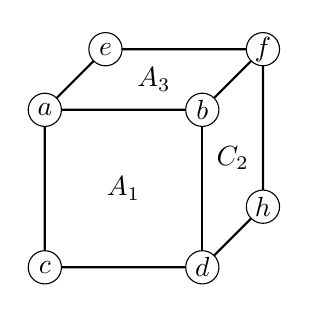
\begin{tikzpicture}
\def\colr{gray!80};

\draw[thick](2,2,0)--(0,2,0)--(0,2,2)--(2,2,2)--(2,2,0)--(2,0,0)--(2,0,2)--(0,0,2)--(0,2,2);
\draw[thick](2,2,2)--(2,0,2);

\node[circle,draw=black,fill=white,minimum size=12pt, label=center:{$a$}] at (0,2,2) {};
\node[circle,draw=black,fill=white,minimum size=12pt, label=center:{$b$}] at (2,2,2) {};
\node[circle,draw=black,fill=white,minimum size=12pt, label=center:{$c$}] at (0,0,2) {};
\node[circle,draw=black,fill=white,minimum size=12pt, label=center:{$d$}] at (2,0,2) {};

\node[circle,draw=black,fill=white,minimum size=12pt, label=center:{$e$}] at (0,2,0) {};
\node[circle,draw=black,fill=white,minimum size=12pt,
label=center:{$f$}] at (2,2,0) {};
\node[circle,draw=black,fill=white,minimum size=12pt, label=center:{$h$}] at (2,0,0) {};

\draw(1,1,2) node{$A_1$};
\draw(1,2,1) node{$A_3$};
\draw(2,1,1) node{$C_2$};

\end{tikzpicture}


\end{document}